
\documentclass[12pt]{article}\usepackage[]{graphicx}\usepackage[]{color}
% maxwidth is the original width if it is less than linewidth
% otherwise use linewidth (to make sure the graphics do not exceed the margin)
\makeatletter
\def\maxwidth{ %
  \ifdim\Gin@nat@width>\linewidth
    \linewidth
  \else
    \Gin@nat@width
  \fi
}
\makeatother

\usepackage{Sweavel}



\usepackage[utf8]{inputenc}
%\usepackage{beamerthemebars}

%\usepackage[spanish]{babel}
\usepackage{fontenc}
\usepackage{graphics}
\usepackage{hyperref}
\usepackage{multimedia}
\usepackage{hyperref}
\usepackage{color}
\usepackage{pgfmath}
\usepackage{tikz}

\usepackage{latexsym} % Símbolos                        ı
\usepackage{amsmath}
\usepackage{amssymb}
\newtheorem{axiom}{Axiom}
\newtheorem{case}{Case}
\newtheorem{claim}{Claim}
\newtheorem{conclusion}{Conclusion}
\newtheorem{condition}{Condition}
\newtheorem{conjecture}{Conjecture}
\newtheorem{assumption}{Assumption}
\newtheorem{propiete}{Propi\'et\'e}
\newtheorem{proposition}{Proposition}
\newtheorem{question}{Question}
\newtheorem{remark}{Remark}


\title{SEIR Epidemiological Model: A Review} 
\author{}
\date{
}

\begin{document}
\maketitle

\section{Basic SIR Model with demography}

Model Assumptions:

\begin{enumerate}
\item The infection circulates in a population of size $N,$ with a per capita background death rate, $\mu$ which is balanced by a birth rate $\mu N$ From the sum of Eqs. (2.1)– (2.3), $\frac{dN}{dt} = 0$ and $N = S + I + R$ is thus constant.
\item The infection causes acute morbidity (not mortality); That is, in this version of the SIR model we assume we can ignore disease-induced mortality. This is reasonable for certain infections like chickenpox, but certainly not for others like rabies, SARS, or ebola.
\item Individuals are recruited directly into the susceptible class at birth (so we ignore perinatal maternal immunity).
\item Transmission of infection from infectious to susceptible individuals is controlled by a bilinear contact term $\beta I S$ This stems from the assumption that the $I$ infectious individuals are independently and randomly mixing with all other individuals, so the fraction $S/N$ of the encounters is with susceptible individuals; $\beta$ is the contact rate times the probability of transmission given a contact between a susceptible and an infectious individual.
\item Chances of recovery or death is assumed not to change during the course of infection.
\item Infectiousness is assumed not to change during the course of infection.
\item Infected individuals move directly into the the infectious class (as opposed to the SEIR model;and remains there for an average infectious period of $1/\gamma$ (assuming $\mu << \gamma$).
\item The model assumes that recovered individuals are immune from reinfection for
life.
\end{enumerate}

The model is characterised taking into account the manifold of Susceptible, Infectious and Recovered individuals, namely
$$
\mathcal{M}_{SIR}(N) = \{(S,I,R) \in \mathbb{R}_+^3 : S+I+R = N\}
$$
together the parameter manifold
$$
\mathcal{P}_{SIR} = \{(\mu,\beta,\gamma) \in \mathbb{R}_+^3: \mu << \gamma\}.
$$
Then for a given an observation $(S_0,I_0,R_0) \in \mathcal{M}_N$ and $(\mu,\beta,\gamma) \in \mathcal{P}_{SIR}$ in time $t=0$ the
evolution of the system is characterised by the ODE:
\begin{align}
\dot{S}(t) & = \mu(N-S)-\beta S \frac{I}{N}, \label{SIR1}\\
\dot{I}(t) & = \beta S \frac{I}{N} - (\mu + \gamma)I, \label{SIR2}\\
\dot{R}(t) & = \gamma I - \mu R \label{SIR3}
\end{align}

For directly transmitted pathogens, $R_0$ is, per definition, the expected number of secondary cases that arise from a typical infectious index-case in a completely susceptible host population. $R_0$ plays a critical role for a number of aspects of disease dynamics and is therefore the focus of much study in historical and contemporary infectious disease dynamics. $(R_0)$ is a very important quantity in epidemiology. For this simple SIR model $$R_0 = \frac{\beta}{\gamma + \mu}$$

We need to load the library to solve numerically an ODE:

\begin{Schunk}
\begin{Sinput}
library(deSolve)
\end{Sinput}
\end{Schunk}

We construct the SIR model function:

\begin{Schunk}
\begin{Sinput}
sirmod = function(t, y, parms) {
  # Pull state variables from y vector
  S = y[1]
  I = y[2]
  R = y[3]
  # Pull parameter values from parms vector beta = parms["beta"]
  mu = parms["mu"]
  gamma = parms["gamma"]
  N = parms["N"]
  beta = parms["beta"]
  # Define equations
  dS = mu * (N - S) - beta * S * I/N
  dI = beta * S * I/N - (mu + gamma) * I 
  dR = gamma * I - mu * R
  res = c(dS, dI, dR)
  # Return list of gradients
  list(res)
}
\end{Sinput}
\end{Schunk}

We introduce the parameter values

\begin{Schunk}
\begin{Sinput}
times = seq(0, 26, by = 1/10)
parms = c(mu = 0.2, N = 1, beta = 2, gamma = 1/2)
start = c(S = 0.999, I = 0.001, R = 0.1)
\end{Sinput}
\end{Schunk}


We integrate numerically \eqref{SIR1}-\eqref{SIR3}

\begin{Schunk}
\begin{Sinput}
out = ode(y=start, times=times, func=sirmod, parms= parms)
out = as.data.frame(out) 
head(round(out, 3))
\end{Sinput}
\begin{Soutput}
  time     S     I     R
1  0.0 0.999 0.001 0.100
2  0.1 0.999 0.001 0.098
3  0.2 0.999 0.001 0.096
4  0.3 0.998 0.001 0.094
5  0.4 0.998 0.002 0.093
6  0.5 0.998 0.002 0.091
\end{Soutput}
\end{Schunk}

Finally, we plot the numerical solution

\begin{Schunk}
\begin{Sinput}
#Calculate R0
R0=parms["beta"]/(parms["gamma"]+parms["mu"])
#Adjust margins to accommodate a second right axis
par(mar = c(5,5,2,5))
#Plot state variables
plot(x=out$time, y=out$S, ylab="Fraction", xlab="Time",type="l")
lines(x=out$time, y=out$I, col="red") 
lines(x=out$time, y=out$R, col="green") 
#Add vertical line at turnover point 
xx = out$time[which.max(out$I)] 
lines(c(xx,xx), c(1/R0,max(out$I)), lty=3)
#prepare to superimpose 2nd plot
par(new=TRUE)
#plot effective reproductive ratio (w/o axes) 
plot(x=out$time, y=R0*out$S, type="l", lty=2, lwd=2,
     col="black", axes=FALSE, xlab=NA, ylab=NA,
ylim=c(-.5, 4.5))
lines(c(xx, 26), c(1,1), lty=3)
#Add right-hand axis for RE
axis(side = 4)
mtext(side = 4, line = 4, expression(R[E])) #Add legend
legend("right", legend=c("S", "I", "R",expression(R[E])), 
	lty=c(1,1,1, 2), col=c("black", "red", "green", "black"))
\end{Sinput}

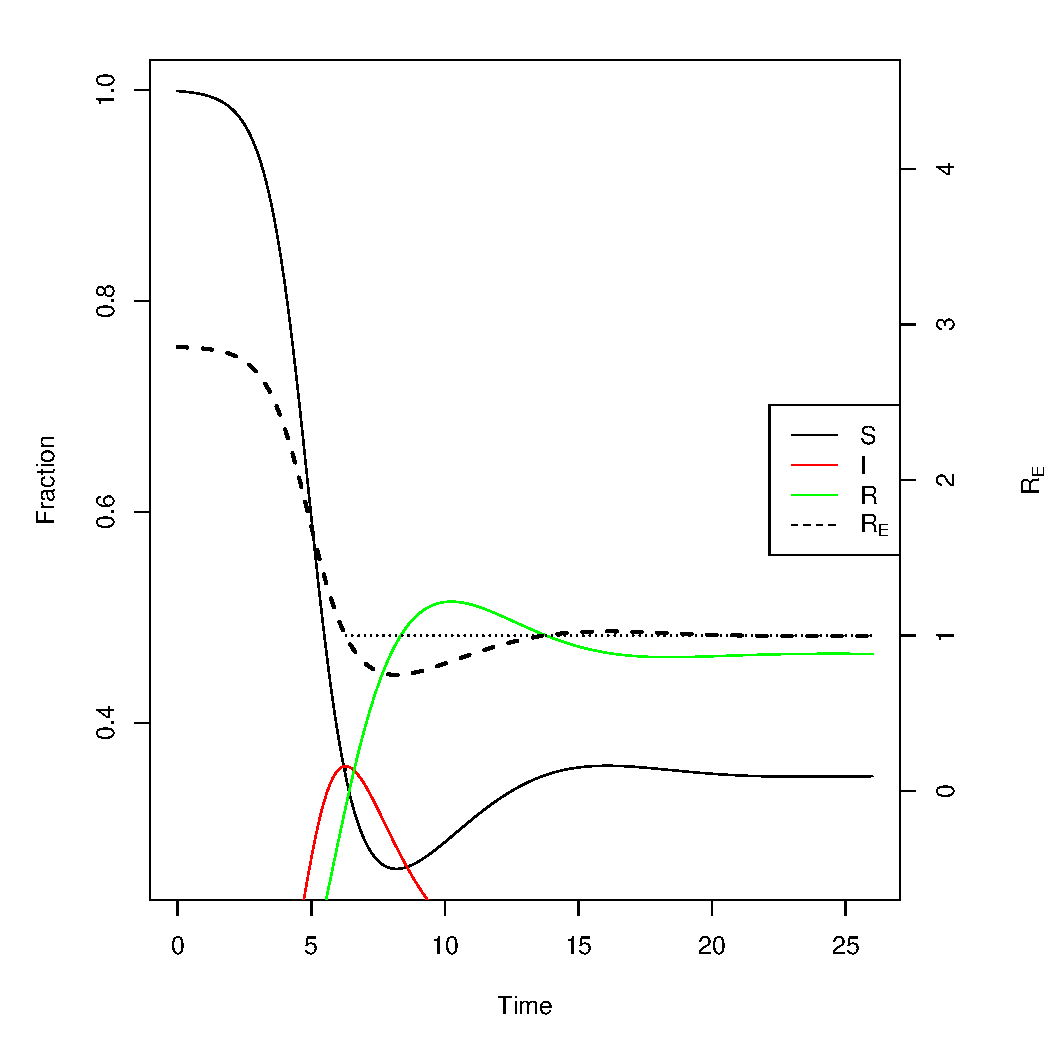
\includegraphics[width=\maxwidth]{figure/unnamed-chunk-5-1} \end{Schunk}


\section{The SEIR Model}

We briefly introduce a refinement to the SIR model to take into account the latent period. The process of transmission often occurs due to an initial inoculation with a very small number of pathogen units (e.g., a few bacterial cells or virions). A period of time then ensues during which the pathogen reproduces rapidly within the host, relatively unchallenged by the immune system. During this stage, pathogen abundance is too low for active transmission to other susceptible hosts, and yet the pathogen is present. Hence, the host cannot be categorized as susceptible, infectious, or recovered; we need to introduce a new category for these individuals who are infected but not yet infectious. These individuals are referred to as Exposed and are represented by the variable $E$ in SEIR models.

We assume that:
\begin{itemize}
\item An average infective individual produces $\beta$ new infections per unit of time when all contacts are with susceptible but that otherwise, this rate is reduced by the ratio $S/N.$
\item Individuals in the exposed class $E$ progress to the infective class at the per capita rate $k.$
\item There is no disease-induced mortality or permanent immunity, and there is a mean infective period of $1/\sigma.$
\end{itemize}
Then the SEIR equations are:
\begin{align}
\dot{S}(t) & = \mu(N-S)-\beta S \frac{I}{N}, \label{SEIR1}\\
\dot{E}(t) & = \beta S \frac{I}{N} - (\mu+\sigma)E, \label{SEIR2} \\
\dot{I}(t) & = \sigma E - (\mu + \gamma)I, \label{SEIR3}\\
\dot{R}(t) & = \gamma I - \mu R \label{SEIR4}
\end{align}
The model is characterised taking into account the manifold of Susceptible, Exposed, Infectious and Recovered individuals, namely
$$
\mathcal{M}_{SEIR}(N) = \{(S,E,I,R) \in \mathbb{R}_+^4 : S+E+I+R = N\}
$$
together the parameter manifold
$$
\mathcal{P}_{SEIR} = \{(\mu,\beta,\gamma,\sigma) \in \mathbb{R}_+^4: \mu << \gamma\}.
$$

We construct the SIR model function:

\begin{Schunk}
\begin{Sinput}
seirmod = function(t, y, parms) {
  # Pull state variables from y vector
  S = y[1]
  E = y[2]
  I = y[3]
  R = y[4]
  # Pull parameter values from parms vector beta = parms["beta"]
  mu = parms["mu"]
  gamma = parms["gamma"]
  N = parms["N"]
  beta = parms["beta"]
  sigma = parms["sigma"]
  # Define equations
  dS = mu * (N - S) - beta * S * I/N
  dE = beta * S * I/N - (mu + sigma) * E
  dI = sigma * E  - (mu + gamma) * I 
  dR = gamma * I - mu * R
  res = c(dS, dE, dI, dR)
  # Return list of gradients
  list(res)
}
\end{Sinput}
\end{Schunk}

We introduce the parameter values

\begin{Schunk}
\begin{Sinput}
times = seq(0, 30, by = 1/10)
parms = c(mu = 0.01, N = 1, beta = 2, gamma = 1/2, sigma = 0.1)
start = c(S = 0.999, E=0.05, I = 0.2, R = 0.1)
\end{Sinput}
\end{Schunk}


We integrate numerically \eqref{SEIR1}-\eqref{SEIR4}

\begin{Schunk}
\begin{Sinput}
out = ode(y=start, times=times, func=seirmod, parms= parms)
out = as.data.frame(out) 
head(round(out, 3))
\end{Sinput}
\begin{Soutput}
  time     S     E     I     R
1  0.0 0.999 0.050 0.200 0.100
2  0.1 0.961 0.088 0.191 0.110
3  0.2 0.926 0.122 0.182 0.119
4  0.3 0.893 0.152 0.175 0.128
5  0.4 0.863 0.181 0.167 0.136
6  0.5 0.836 0.206 0.161 0.144
\end{Soutput}
\end{Schunk}

Finally, we plot the numerical solution

\begin{Schunk}
\begin{Sinput}
#Calculate R0
R0=(parms["beta"]*parms["sigma"])/
((parms["gamma"]+parms["mu"])*(parms["sigma"]+parms["mu"]))
#Adjust margins to accommodate a second right axis
par(mar = c(5,5,2,5))
#Plot state variables
plot(x=out$time, y=out$S, ylab="Fraction", xlab="Time",type="l")
lines(x=out$time, y=out$E, col="purple") 
lines(x=out$time, y=out$I, col="red") 
lines(x=out$time, y=out$R, col="green") 
#Add vertical line at turnover point 
xx = out$time[which.max(out$I)] 
lines(c(xx,xx), c(1/R0,max(out$I)), lty=3)
#prepare to superimpose 2nd plot
par(new=TRUE)
#plot effective reproductive ratio (w/o axes) 
plot(x=out$time, y=R0*out$S, type="l", lty=2, lwd=2,
     col="black", axes=FALSE, xlab=NA, ylab=NA,
ylim=c(-.5, 4.5))
lines(c(xx, 26), c(1,1), lty=3)
#Add right-hand axis for RE
axis(side = 4)
mtext(side = 4, line = 4, expression(R[E])) #Add legend
legend("topright", legend=c("S","E" ,"I", "R",expression(R[E])), 
  lty=c(1,1,1,1,2), col=c("black","purple" , "red", "green", "black"))
\end{Sinput}

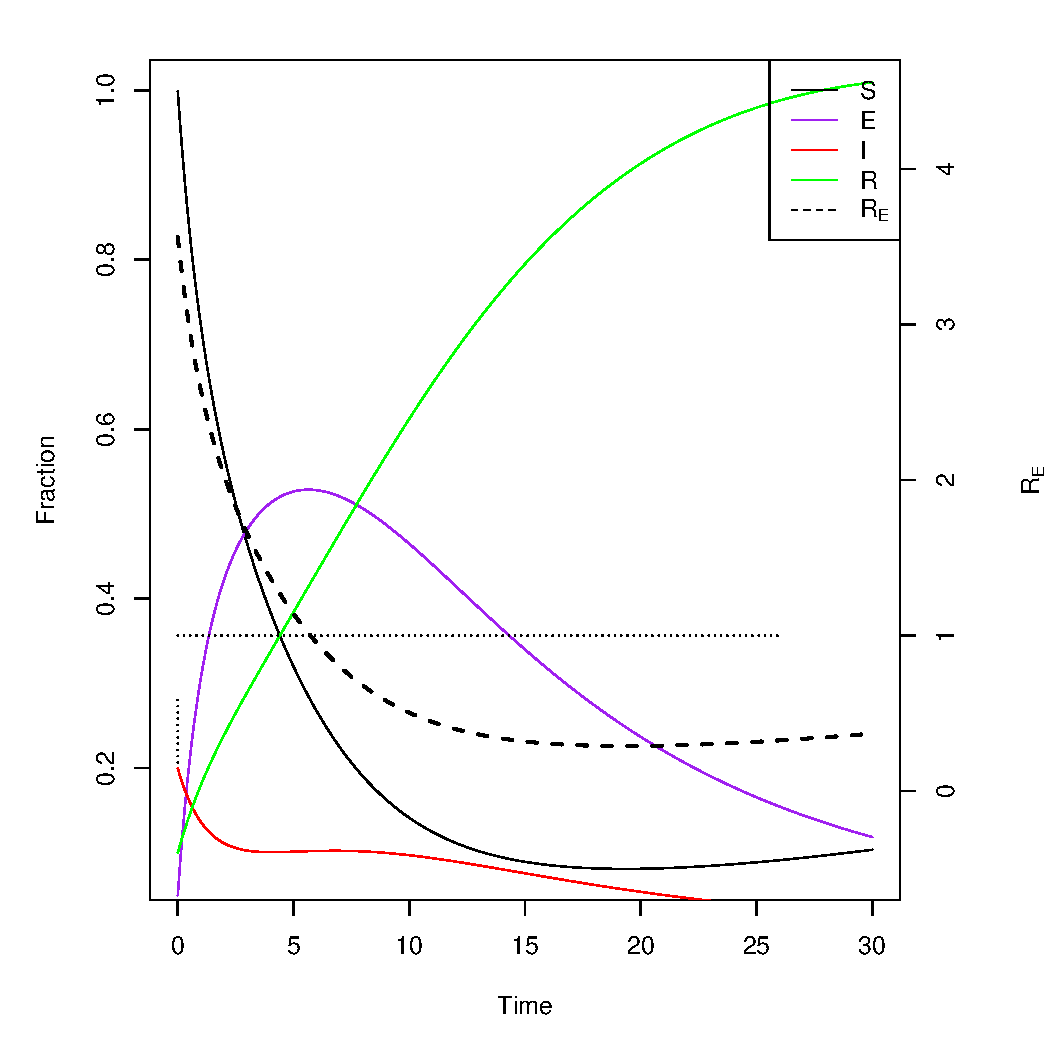
\includegraphics[width=\maxwidth]{figure/unnamed-chunk-9-1} \end{Schunk}

\end{document}
